% Created 2021-03-11 Thu 12:00
% Intended LaTeX compiler: pdflatex
\documentclass[english]{article}
\usepackage[T1, T2A]{fontenc}
\usepackage[lutf8]{luainputenc}
\usepackage[english, russian]{babel}
\usepackage{minted}
\usepackage{graphicx}
\usepackage{longtable}
\usepackage{hyperref}
\usepackage{xcolor}
\usepackage{natbib}
\usepackage{amssymb}
\usepackage{stmaryrd}
\usepackage{amsmath}
\usepackage{caption}
\usepackage{mathtools}
\usepackage{amsthm}
\usepackage{tikz}
\usepackage{grffile}
\usepackage{extarrows}
\usepackage{wrapfig}
\usepackage{rotating}
\usepackage{placeins}
\usepackage[normalem]{ulem}
\usepackage{amsmath}
\usepackage{textcomp}
\usepackage{capt-of}

\usepackage{geometry}
\geometry{a4paper,left=2.5cm,top=2cm,right=2.5cm,bottom=2cm,marginparsep=7pt, marginparwidth=.6in}

 \usepackage{hyperref}
 \hypersetup{
     colorlinks=true,
     linkcolor=blue,
     filecolor=orange,
     citecolor=black,      
     urlcolor=cyan,
     }

\usetikzlibrary{decorations.markings}
\usetikzlibrary{cd}
\usetikzlibrary{patterns}

\newcommand\addtag{\refstepcounter{equation}\tag{\theequation}}
\newcommand{\eqrefoffset}[1]{\addtocounter{equation}{-#1}(\arabic{equation}\addtocounter{equation}{#1})}


\newcommand{\R}{\mathbb{R}}
\renewcommand{\C}{\mathbb{C}}
\newcommand{\N}{\mathbb{N}}
\newcommand{\rank}{\text{rank}}
\newcommand{\const}{\text{const}}
\newcommand{\grad}{\text{grad}}

\theoremstyle{plain}
\newtheorem{axiom}{Аксиома}
\newtheorem{lemma}{Лемма}
\newtheorem{manuallemmainner}{Лемма}
\newenvironment{manuallemma}[1]{%
  \renewcommand\themanuallemmainner{#1}%
  \manuallemmainner
}{\endmanuallemmainner}

\theoremstyle{remark}
\newtheorem*{remark}{Примечание}
\newtheorem*{solution}{Решение}
\newtheorem{corollary}{Следствие}[theorem]
\newtheorem*{examp}{Пример}
\newtheorem*{observation}{Наблюдение}

\theoremstyle{definition}
\newtheorem{task}{Задача}
\newtheorem{theorem}{Теорема}[section]
\newtheorem*{definition}{Определение}
\newtheorem*{symb}{Обозначение}
\newtheorem{manualtheoreminner}{Теорема}
\newenvironment{manualtheorem}[1]{%
  \renewcommand\themanualtheoreminner{#1}%
  \manualtheoreminner
}{\endmanualtheoreminner}
\captionsetup{justification=centering,margin=2cm}
\newenvironment{colored}[1]{\color{#1}}{}

\tikzset{->-/.style={decoration={
  markings,
  mark=at position .5 with {\arrow{>}}},postaction={decorate}}}
\makeatletter
\newcommand*{\relrelbarsep}{.386ex}
\newcommand*{\relrelbar}{%
  \mathrel{%
    \mathpalette\@relrelbar\relrelbarsep
  }%
}
\newcommand*{\@relrelbar}[2]{%
  \raise#2\hbox to 0pt{$\m@th#1\relbar$\hss}%
  \lower#2\hbox{$\m@th#1\relbar$}%
}
\providecommand*{\rightrightarrowsfill@}{%
  \arrowfill@\relrelbar\relrelbar\rightrightarrows
}
\providecommand*{\leftleftarrowsfill@}{%
  \arrowfill@\leftleftarrows\relrelbar\relrelbar
}
\providecommand*{\xrightrightarrows}[2][]{%
  \ext@arrow 0359\rightrightarrowsfill@{#1}{#2}%
}
\providecommand*{\xleftleftarrows}[2][]{%
  \ext@arrow 3095\leftleftarrowsfill@{#1}{#2}%
}
\makeatother
\author{Ilya Yaroshevskiy}
\date{\today}
\title{Практика 5}
\hypersetup{
 pdfauthor={Ilya Yaroshevskiy},
 pdftitle={Практика 5},
 pdfkeywords={},
 pdfsubject={},
 pdfcreator={Emacs 28.0.50 (Org mode )}, 
 pdflang={English}}
\begin{document}

\maketitle
\tableofcontents

\[ f \ge 0\quad \int_\Omega f d\mu \]
\[ f\text{ --- суммируемая } \int_\Omega|f|d\mu < + \infty \]

\begin{examp}
\[ f = \frac{1}{x^2 + y^2} \]
\(\Omega\) --- окружность радиуса \(1\)
\[ \iint \frac{1}{x^2 + y^2} dx dy = \sum_n \iint \frac{1}{x^2 + y^2} dx dy \asymp \sum \addtag\label{5_1_sum}\]
\color{blue}
\[ f, g > 0\quad f\asymp g \quad \exists c_1, c_2 > 0\ c_1f < g < c_2f \]
\[ \inf f\mu E \le \int_E f d\mu \le \sup f \mu E \]
\color{black}
\begin{center}
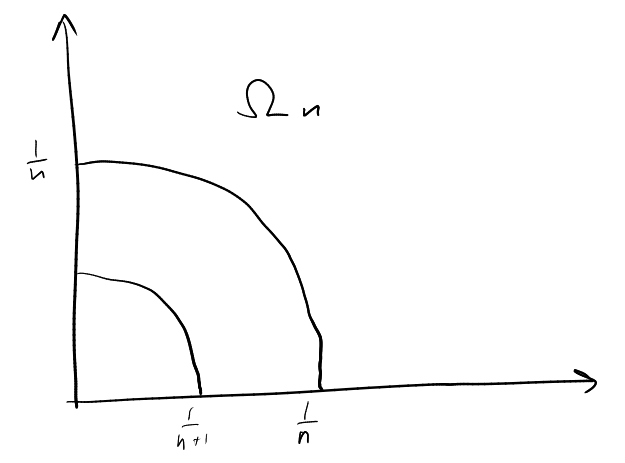
\includegraphics[scale=0.4]{5_1.png}
\end{center}
в \(\Omega_n\):
\[ \frac{1}{x^2 + y^2} \asymp \frac{1}{\frac{1}{n^2}} \]
\[ \frac{1}{\frac{1}{n^2}} \le \frac{1}{x^2 + y^2} \le \frac{1}{\frac{1}{(n + 1)^2}} \]
\[ n^2 \le \frac{1}{x^2 + y^2} \le (n + 1)^2 \le 4n^2 \]
\[ (\text{продолжение }\ref{5_1_sum})\ \sum_{n = 1}^{ + \infty} n^2 \cdot \lambda \Omega_n = \sum n^2 \frac{\pi}{4} \left(\frac{1}{n^2} - \frac{1}{(n + 1)^2}\right) \sim \sum \frac{c}{n}\text{ --- расходится}\]
\end{examp}
\begin{examp}
\[ f = \frac{1}{x + y} \]
\(\Omega\) --- квадрат \(1\times 1\)
\[ \iint \frac{1}{x + y} = \sum_{n = 1}^{ + \infty}\iint \frac{1}{x + y} \asymp \sum \frac{1}{\frac{1}{n}} \addtag\label{5_2_sum}\]
\begin{center}
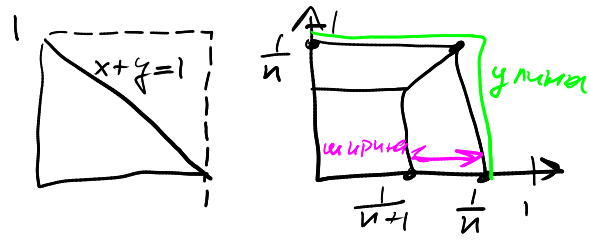
\includegraphics[scale=0.4]{5_2.png}
\end{center}
\[ \frac{1}{2}\cdot\frac{1}{n} \le \frac{1}{n + 1} < x+ y \le \frac{2}{n} \]
\[ \ref{5_2_sum} \sum \frac{1}{\frac{1}{n}}\cdot \frac{1}{n^3} = \sum \frac{1}{n^2}\text{ --- сходится} \]
длина \(\approx \frac{1}{n}\), 
ширина \(\approx \frac{1}{n^2}\)
\end{examp}


Функции:
\begin{enumerate}
\item \[ f(x, y) = \frac{1}{(x^2 + y^2)^p} \]
\item \[ g(x, y) = \frac{1}{|x + y|^p} \]
\item \[ h(x, y) = \frac{1}{|1 - x^2 - y^2|^p} \]
\end{enumerate}


Области:
\begin{figure}[H]
\centering
\begin{minipage}{20em}
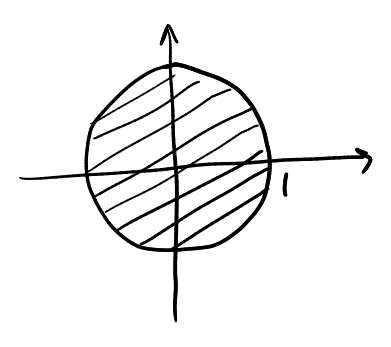
\includegraphics[scale=0.3]{5_3.png}
\caption{Круг}
\end{minipage}
\begin{minipage}{20em}
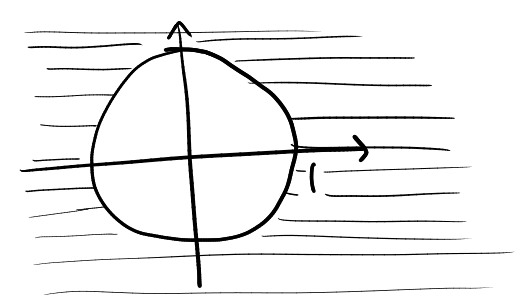
\includegraphics[scale=0.3]{5_4.png}
\caption{Доплнение круга}
\end{minipage}
\end{figure}

\begin{figure}[H]
\centering
\begin{minipage}{20em}
\centering
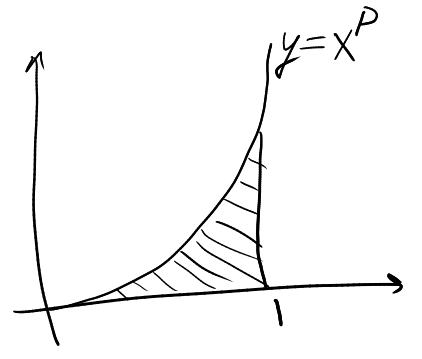
\includegraphics[scale=0.3]{5_5.png}
\caption{Треугольник}
\end{minipage}
\begin{minipage}{20em}
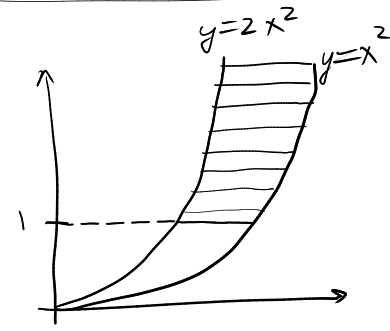
\includegraphics[scale=0.3]{5_7.png}
\caption{"Рог"}
\end{minipage}
\end{figure}

\begin{figure}[H]
\centering
\begin{minipage}{20em}
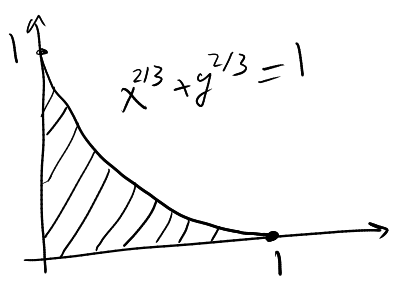
\includegraphics[scale=0.3]{5_6.png}
\caption{Четверть астроиды}
\end{minipage}
\begin{minipage}{20em}
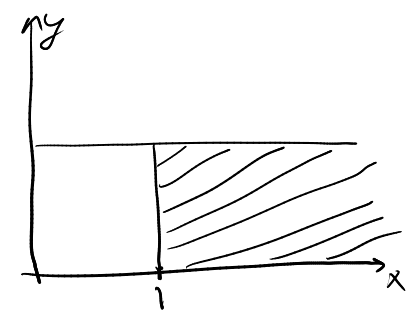
\includegraphics[scale=0.3]{5_8.png}
\caption{Полоса}
\end{minipage}
\end{figure}

\begin{task}
\(f\) = 1., Дополнение круга
\end{task}
\begin{solution}
\[ \frac{1}{(n + 1)^{2p}} \le f \le \frac{1}{n^{2p}} \Rightarrow f \asymp \frac{1}{n^{2p}} \]
\[ \frac{1}{(n + 1)^{2p}} \le f \le \frac{1}{n^{2p}} \Rightarrow f \asymp \frac{1}{n^{2p}} \]
\[ \iint \frac{dx dy}{(x^2 + y^2)^p} = \sum_{n = 1}^{ + \infty} \iint_{\Omega_n} \frac{1}{(x^2 + y^2)^p} \asymp \sum \frac{1}{n^2 p} \cdot n = \sum \frac{1}{n^{2p - 1}} \]
\begin{itemize}
\item \(2p - 1 > 1\) --- сходится
\item \(2p - 1\le 1\) --- расходится
\end{itemize}
\end{solution}
\begin{task}
\(f\) = 3., Круг
\end{task}
\begin{solution}
\[ \iint_\Omega f = \sum_n \iint_{\Omega_n}\frac{1}{|1 - x^2 - y^2|^p} dx dy \addtag\label{5_3}\]
\begin{center}
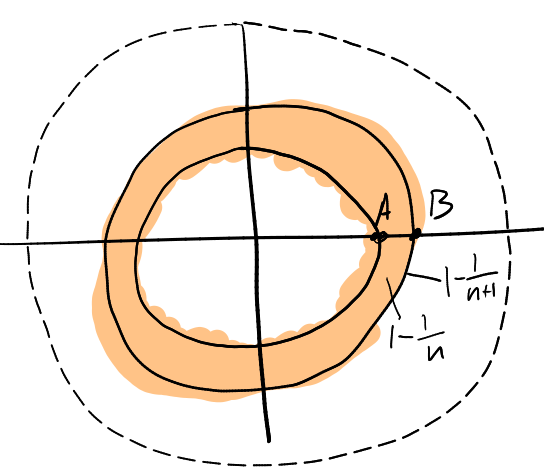
\includegraphics[scale=0.4]{5_9.png}
\end{center}
\begin{description}
\item[{A:}] \[ 1 - (1 - \frac{1}{n})^2 - o^2 = \frac{2}{n} - \frac{1}{n^2} \]
\item[{B:}] \[ \frac{2}{n + 1} - \frac{1}{(n + 1)^2} \]
\end{description}
\[ \frac{1}{2n} < \frac{1}{n + 1} < \frac{2}{n + 1} - \frac{1}{(n + 1)^2} \le 1 - (x^2 + y^2) \le 1 - \left(1 - \frac{1}{n}\right)^2 \le \frac{2}{n} \]
\[ 1 - (x^2 + y^2) \asymp \frac{1}{n} \]
\[ f \asymp \frac{1}{\left(\frac{1}{n}\right)^p} = n^p \]
\[ \ref{5_3} \asymp \sum n^p\cdot\frac{1}{n^2} = \sum \frac{1}{n^{2 - p}} \]
\begin{itemize}
\item \(2 - p > 1\) --- сходится
\item \(2 - p < 1\) --- расходится
\end{itemize}
\end{solution}
\begin{task}
\(f\) = 2., "Рог"
\end{task}
\begin{solution}
\[ \iint_\Omega f = \sum_n \iint_{\Omega_n} \addtag\label{5_4} \]
\begin{center}
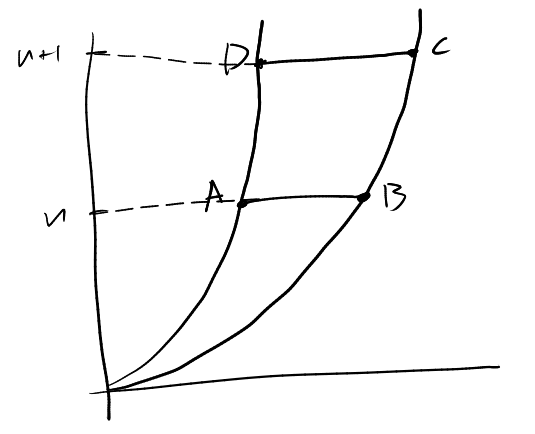
\includegraphics[scale=0.3]{5_10.png}
\end{center}
\begin{description}
\item[{\(x + y\):}] \-
\begin{center}
\begin{tabular}{llll}
\(A\left(\sqrt{\frac{n}{2}}, 2\right)\) & \(n + \frac{\sqrt{n}}{\sqrt{2}}\) & D & \(n + 1 + \frac{\sqrt{n + 1}}{\sqrt{2}}\)\\
\(B(\sqrt{n}, n)\) & \(n + \sqrt{n}\) & C & \(n + 1 + \sqrt{n + 1}\)\\
\end{tabular}
\end{center}
\end{description}
\[ \frac{1}{(3n)^p} \le "D" \frac{1}{(x + y)^p} \le "A" \frac{1}{\left(n + \frac{\sqrt{n}}{\sqrt{2}}\right)^p} \le \frac{1}{n^p} \]
\[ f \asymp \frac{1}{n^p} \]
\[ \ref{5_4} \asymp \sum \frac{1}{n^p}\cdot\sqrt{n} = \sum \frac{n^{p - \frac{1}{2}}}\]
\begin{itemize}
\item \(p - \frac{1}{2} > 1\) --- сходится
\item \(p - \frac{1}{2} \le 1\) --- расходится
\end{itemize}
\end{solution}
\begin{task}
\(f\) = 1., "Рог"
\end{task}
\begin{solution}
\[ \iint_\text{"Рог"}\frac{1}{(x^2 + y^2)^p} = \sum \int_{\Omega_n} \asymp \sum \frac{1}{n^2p}\cdot\sqrt{n} \]
\end{solution}
\end{document}
